\chapter{Standortplanung in der Ebene} % (fold)
\label{cha:standortplanung_in_der_ebene}

  \section{Theorie der Standortplanung} % (fold)
  \label{sec:theorie_der_standortplanung}

    \par \textbf{Grundlegende Aufgabenstellung}
    \par Platzierung ein oder mehrerer neuer Einrichtungen in Abhängigkeit bereits existierender Einrichtungen

    \par Drei Klassen von Standortproblemen:
    \begin{itemize}
      \item \textbf{Standortprobleme in der Ebene} (Einfachste, allerdings auch unrealistichste Problemklasse)
      \item \textbf{Standortprobleme auf Netzwerken} (praxisbezug viel ausgeprägter als bei planaren Standortproblemen)
      \item \textbf{Diskrete Standortprobleme} (realistischste und flexibelste Klasse von Standortproblemen)
    \end{itemize}
  
  % section theorie_der_standortplanung (end)

  \section{Begriffe und Notationen} % (fold)
  \label{sec:begriffe_und_symbole}

    \begin{defn}
      \textbf{Standorte}
      als Punkte idealisiert
    \end{defn}

    \begin{defn}
      \textbf{Neue Einrichtungen $X = {x_1, \dots, x_p}, p \geq 1$}
      \begin{itemize}
        \item dürfen überall in der Ebene platziert werden
        \item ihre Standorte werden durch Koordinaten repräsentiert
        \[ x_i = (x_{i, 1}, x_{i, 2}) \in \mathbb{R}^{2}, \forall i = 1, \dots, p\]
      \end{itemize}
    \end{defn}

    \begin{defn}
      \textbf{Existierende Einrichtungen (Kunden) $A = {a_1, \dots, a_n}$}
      \begin{itemize}
        \item werden durch eine Menge von Punkten in der Ebene repräsentiert
        \[ a_i = (a_{i, 1}, a_{i, 2}) \in \mathbb{R}^2, \forall i = 1, \dots, n\] 
        \item Jedem Kunden $a_i \in A$ wird ein positives Gewicht $w_i > 0$ zugeordnet.
      \end{itemize}
    \end{defn}
    
    \begin{defn}
      \textbf{Kosten}\\
      Lediglich Transportkosten werden berücksichtigt. Sie sind proportional zur Menge und zur zurückgelegten Entfernung.
    \end{defn}
    

    \subsection{Distanzmessung} % (fold)
    \label{sub:distanzmessung}

      \begin{defn}
        \textbf{Metrik / Distanzfunktion}
        $$d: \mathbb{R}^n \times \mathbb{R}^n \rightarrow \mathbb{R}$$
      \end{defn}
      \par welche für alle $ x, y, z \in \mathbb{R}^n, n \geq 1$ folgende Eigenschaften erfüllt: 
      \begin{itemize}
            \item Definitheit: $d(x,y) \geq 0 \text{ und } d(x, y) = 0 \Leftrightarrow x = y$
            \item Symmetrie: $d(x,y) = d(y, x)$
            \item Dreiecks-Ungleichung: $d(x, y) \leq d(x, z) + d(z, y)$
          \end{itemize}
    
    % subsection distanzmessung (end)

    \subsection{$l_p$-Metrik} % (fold)
    \label{sub:lp_metrik}

    \begin{equation}
      l_p(x, y) = \sqrt[p]{|x_1 - y_1| ^ p + |x_2 - y_2| ^ p}, p \geq 1
    \end{equation}
    \par \textbf{Rechtwinklige Entfernung ($l_1-$ oder Manhatten-Metrik)}

    \begin{equation}
      l_1(x, y) = |x_1 - y_1| + |x_2 - y_2|
    \end{equation}

    \par \textbf{Euklidische Entfernung ($l_2-$ oder Luftlinien-Metrik)}

    \begin{equation}
      l_2(x, y) = \sqrt{|x_1 - y_1| ^ 2 + |x_2 - y_2| ^ 2}
    \end{equation}

    \par \textbf{Quadrierte euklidische Entfernung ($l_2^2-$-Metrik)}

    \begin{equation}
      l_2(x, y) = |x_1 - y_1| ^ 2 + |x_2 - y_2| ^ 2
    \end{equation}


    \par \textbf{Tchebychev Entfernung ($l_\infty$-Metrik)}
    \begin{equation}
      l_{\infty}(x, y) = \text{max}\{\left|x_1 - y_1\right|, \left|x_2 - y_2\right|\}
    \end{equation}
    
    % subsection lp_metrik (end)

  % section begriffe_und_symbole (end)

  \section{1-Medianprobleme} % (fold)
  \label{sec:1_medianprobleme}

    \subsection{Einleitung} % (fold)
    \label{sub:einleitung}

      \subsubsection{Aufgabe} % (fold)
      \label{ssub:aufgabe}
    
      \par Platziere eine neue Einrichtung so in der Ebene, dass die Summe der gewichteten Entfernungen von dem neuen Standort zu allen Kunden minimal wird.

      \begin{equation}
        \underset{x \in \mathbb{R}^2}{\text{min}} f(x) := \sum_{i = 1}^{n}w_id(x, a_i) 
      \end{equation}

      \begin{itemize}
        \item $A = {a_1, \dots, a_n}:$ die $n$ Kunden
        \item $w_i > 0, i = 1, \dots, n$: die damit assoziierten Gewichte
        \item $x$: der gesuchte Standort der neuen Einrichtung 
        \item $d$: eine Metrik
      \end{itemize}

      \par Nenne einen Punkt $x^* \in \mathbb{R}^2$, welcher die Funktion $f(x)$ minimiert ($f(x^*) \leq f(x), \forall x \in \mathbb{R}^2$), \textbf{optimal}.

      \par Bezeichne die Menge aller optimalen Punkte der Funktion $f(\cdot)$ mit $\mathcal{X}^*(f)$.

      % subsubsection aufgabe (end)

      \subsubsection{Dominanzkriterium} % (fold)
      \label{ssub:dominanzkriterium}

        \par Gilt für einen Kunden $a_k$ mit zugehörigem Geweicht $w_k$, dass 
        \[w_k \geq \frac{1}{2}\sum_{i=1}^{n}w_i ,\]
        d. h. der Kunde vereinigt mindestens die Hälfte aller Gewichte auf sich, so ist der Standort des Kunden $a_k$ eine optimale Lösung des Problems.
      
      % subsubsection dominanzkriterium (end)

    % subsection einleitung (end)

    \subsection{1-Medianprobleme mit $l_1$-Metrik} % (fold)
    \label{sub:1_medianprobleme_mit_l1_Metrik}
    
      \par \textbf{Zielfunktion}

      \begin{equation}
        \begin{aligned}
            f(x) &= \sum_{i=1}^{n}w_il_1(x, a_i) \\
                 &= \sum_{i=1}^{n}w_il_1(\left|x_1 - a_{i,1}\right| + \left|x_2 - a_{i,2}\right|) \\
                 &= \underbrace{\sum_{i=1}^{n}w_il_1(\left|x_1 - a_{i,1}\right|)}_{=: f_1(x_1)} + \underbrace{\sum_{i=1}^{n}w_il_1(\left|x_2 - a_{i,2}\right|}_{=:f_2(x_2)}
        \end{aligned}
      \end{equation}

      $\rightarrow$ Die ursprüngliche Aufgabe reduziert sich auf das Lösen zweier 1-dimensionaler Probleme, sogenannter ``Probleme auf der Linie''.

      \subsubsection{Das 1-Medianproblem mit $l1$-Metrik auf der Linie} % (fold)
      \label{ssub:das_1_medianproblem_mit_metrik_auf_der_linie}
      
      \[\underset{x \in \mathbb{R}}{\text{min}} f(x) := \sum_{i= 1}{n}w_i\left|x - a_i\right|\]

      \begin{algorithm}[H]
        \caption{Lösungsverfahren für das 1-Medianproblem mit $l1$-Metrik auf der Linie}
        % \textbf{Input}: Anzahl Suchrichtungen $K, \beta, V, p$
        \begin{algorithmic}[1]
          % \Procedure{MyProcedure}{}
          \State Berechne die Summe $W$ aller Gewichte $W:=\sum_{i= 1}{n}w_i$
          \If (Es exist. ein $w_k \geq \frac{1}{2}W$)
            \State Der Kundenstandort $a_k$ ist eine optimale Lösung, $x^* = a_k$
            \State Stopp
          \Else
            \State Sortiere die Kundenstandorte $a_1, \dots, a_n$ nach monoton wachsenden Koordinaten $a_{i_1} \leq a_{i_2} \leq \dots \leq a_{i_n}$
            \State Bestimme unter Berücksichtigung einer zu den Kundenstandorten analogen Sortierung der Gewichte dasjenige $h$, für welches folgendes gilt:
            \[\sum_{j=1}^{h-1}w_{i_j} < \frac{1}{2}W \text{ und } \sum_{j=1}^{h}w_{i_j} \geq \frac{1}{2}W\] (die Gewichte der Reihe nach so lange aufsummiert, bis diese Summe gerade eben mehr als die Hälfte der gesamten Gewichte umfasst.)
            \State $x^* = a_{i_h}$ ist die Koordinate eines optimalen Standorts, d.h. $\mathcal{X}^*(f) = \left\{a_{i_h}\right\}$
          \EndIf
          % \EndProcedure
        \end{algorithmic}
        % \textbf{Output:} 
      \end{algorithm}

      \begin{exmp}
        
      \end{exmp}

      \begin{figure}[H]
        \centering
        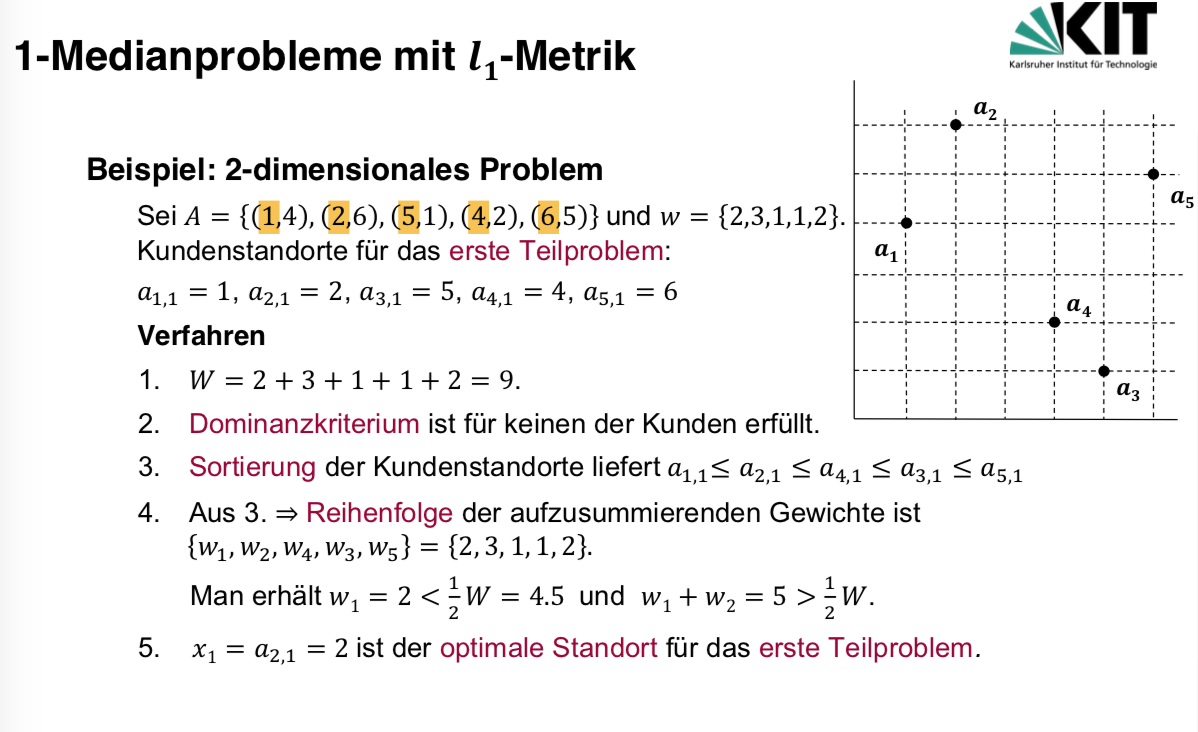
\includegraphics[width=0.95\textwidth]{Images/das_1_medianproblem_mit_metrik_auf_der_linie_Bsp(1).png}
        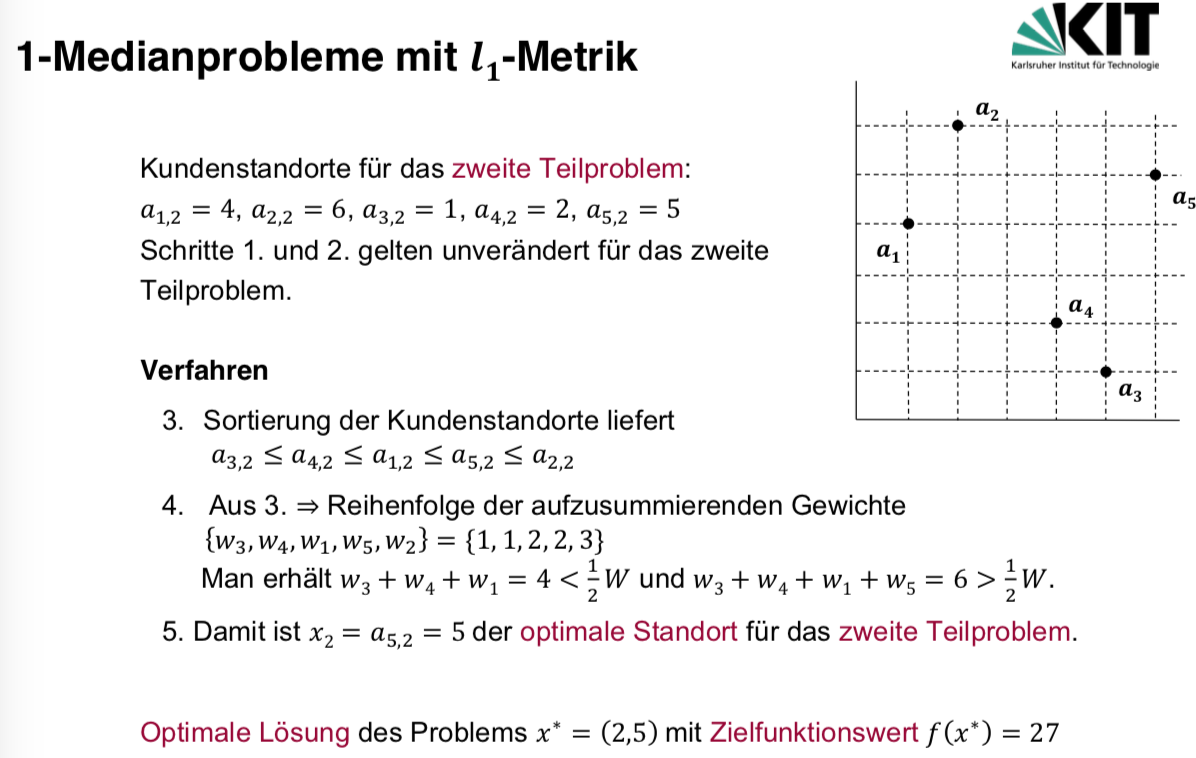
\includegraphics[width=0.95\textwidth]{Images/das_1_medianproblem_mit_metrik_auf_der_linie_Bsp(2).png}
        \caption{das $1$ medianproblem mit metrik auf der linie}
        \label{fig:das_1_medianproblem_mit_metrik_auf_der_linie}
      \end{figure}

      \textbf{Restriktive Standortprobleme mit verbotenes Gebiet R}

      \par potentielle Standorte: Schnittpunkte der achsenparallelen Geraden durch Kunden mit verboten Gebiet

      \begin{exmp}
        \color{blue}{Aufgabe 7(b)}
      \end{exmp}


      % subsubsection das_1_medianproblem_mit_metrik_auf_der_linie (end)

    % subsection 1_medianprobleme_mit_ (end)

    \subsection{1-Medianprobleme mit ${l_2}^{2}$-Metrik} % (fold)
    \label{sub:1_medianprobleme_mit_l2^2_Metrik}

    \par \textbf{Zielfunktion}

    \begin{equation}
      \begin{aligned}
        f(x) &= \sum_{i=1}^{n}w_{i}l_{2}^{2}(x, a_i) \\
             &= \sum_{i=1}^{n}w_{i}l_{2}^{2}((x_1 - a_{i, 1})^2 + (x_2 - a_{i,2})^2) \\
             &= \sum_{i=1}^{n}w_{i}l_{2}^{2}(x_1 - a_{i, 1})^2 + \sum_{i=1}^{n}w_{i}l_{2}^{2}(x_2 - a_{i, 2})^2 \\
             &=: f_1(x_1) + f_2(x_2)
      \end{aligned}
    \end{equation}

    \par $f_1(x_1)$ und $f_2(x_2)$ sind differenzierbar.

    \par Ableiten nach $x_1$ bzw. $x_2$ und Nullsetzen der jeweiligen Ableitung ergibt:

    \begin{equation*}
      \underbrace{x^*}_{Schwerpunkt} = \left(\frac{\sum_{i=1}^{n}w_ia_{i,1}}{\sum_{i=1}^{n}w_i}, \frac{\sum_{i=1}^{n}w_ia_{i,2}}{\sum_{i=1}^{n}w_i} \right)
    \end{equation*}
    
    % subsection 1_medianprobleme_mit_ (end)

    \subsection{1-Medianprobleme mit $l_2$-Metrik} % (fold)
    \label{sub:1_medianprobleme_mit_l2_Metrik}

      \par \textbf{Zielfunktion}
      \begin{equation}
        f(x) = \sum_{i=1}^{n}w_il_2(x, a_i) = \sum_{i=1}^{n}w_i\sqrt{(x_1 - a_{i,1})^2 + (x_2 - a_{i,2})^2}
      \end{equation}

      \par Die Zielfunktion ist nicht zerlegbar!

      \par \textbf{Verschärftes Dominanzkriterium}

      \par Der Standort $a_j$ eines Kunden ist optimal, falls

      \begin{equation}
        \gamma(a_j) := l_2(\sum_{i=1, i \neq j} w_i \frac{a_j - a_i}{l2(a_j, a_i)}, \mathbf{0}) \leq w_j, \mathbf{0} = (0, 0)
      \end{equation}


      \begin{algorithm}[htbp]
        \caption{Das Approximations-Verfahren von Weiszfeld}
        % \textbf{Input}: Anzahl Suchrichtungen $K, \beta, V, p$
        \begin{algorithmic}[1]
          % \Procedure{MyProcedure}{}
          \If {(Verschärftes Dominanzkriterium $\gamma(a_j) \leq w_j$ erfüllt)}
            \State $x^* = a_j$, \textbf{STOPP!}
          \Else
            \State $k:=0$
            \State $x^{(0)}:=\frac{\sum_{i=1}^{n}w_ia_i}{\sum_{i=1}^{n}w_i}$ (Schwerpunkt)
            \While {($\text{!}(\delta^(k+1):= \frac{f(x^{(k)}) - f(x^{(k+1)})}{f(x^{(k)})} \leq \delta$)}
              \State $x^{(k+1)} := \frac{\sum_{i=1}^{n}w_i\frac{a_i}{l_2(x^{(k)}, a_i)}}{\sum_{i=1}^{n}w_i\frac{1}{l_2(x^{(k)}, a_i)}}$
              \State $k:=k+1$
            \EndWhile
          \EndIf
          % \EndProcedure
        \end{algorithmic}
        % \textbf{Output:} 
      \end{algorithm}

          
    % subsection 1_medianprobleme_mit_ (end)
  
  % section 1_medianprobleme (end)

  \section{1-Centerprobleme} % (fold)
  \label{sec:1_centerprobleme}

    \subsection{Aufgabe} % (fold)
    \label{sub:aufgabe}

      Platziere eine neue Einrichtung so in der Ebene, dass die maximale gewichtete Entfernung von dem neuen Standort zu den Kunden minimal wird.
    
    % subsection aufgabe (end)

    \subsection{formel} % (fold)
    \label{sub:formel}
      \begin{equation}
        \underset{x \in \mathbb{R}^2}{\text{min}}g(x) \text{ mit } g(x) := \underset{i = 1, \dots, n}{\text{max}}w_id(x, a_i)
      \end{equation}
    % subsection formel (end)

    \subsection{1-Centerprobleme mit $l_1$-Metrik} % (fold)
    \label{sub:1_centerprobleme_mit_l_1_metrik}

      \par \textbf{Zielfunktion}

      \begin{equation}
        \begin{aligned}
          g(x) &= \underset{i = 1, \dots, n}{\text{max}}w_il_1{x, a_i} \\
               &= \underset{i = 1, \dots, n}{\text{max}}w_i(\left|x_1 - a_{i, 1} \right| + \left| x_2 - a_{i,2}\right|)
        \end{aligned}
      \end{equation}

      \begin{algorithm}[htbp]
        \caption{Lösungsverfahren für das $l_1$-Centerproblem}
        % \textbf{Input}: Anzahl Suchrichtungen $K, \beta, V, p$
        \begin{algorithmic}[1]
          % \Procedure{MyProcedure}{}
          \State Transformiere alle Kundenstandorte mit 
            \[
              T = \begin{pmatrix}
                1 & -1 \\
                1 & 1 
              \end{pmatrix}
            \]          
          \State Finde eine optimale Lösung $x_{\infty}^{*}$ des $l_{\infty}$-Problems mit den Kundenstandorten $A'$
          \State Erhalte eine optimale Lösimg $x^{*}$ des $l_1$-Problems: 
            \[
              x^* = x_{\infty}^* \cdot T^{-1}
            \]
          % \EndProcedure
        \end{algorithmic}
        % \textbf{Output:} 
      \end{algorithm}

      \subsubsection{1-Centerprobleme mit $l_{\infty}$-Metrik} % (fold)
      \label{ssub:_1_centerprobleme_mit_}

        \par \textbf{Zielfunktion}

        \begin{equation}
          \begin{aligned}
            g(x) &= \underset{i = 1, \dots, n}{\text{max}}w_il_{\infty}(x, a_i) \\
                 &= \underset{i = 1, \dots, n}{\text{max}}w_i(\left| x_1 - a_{i,1}\right|, \left| x_2 - a_{i,2}\right|)  
          \end{aligned}
        \end{equation}

        \subsubsubsection{Der ungewichtete Fall}

          \par Umformulierung des Problems:

          \begin{equation*}
            \underset{x \in \mathbb{R}^2}{\text{min}} \underset{i = 1, \dots, n}{\text{max}}l_{\infty}(x, a_i) \Leftrightarrow \underset{}{\text{min } z}, \text{u.d.N } l_{\infty}(x, a_i) \leq z, \forall i = 1, \dots, n
          \end{equation*}

          $\Rightarrow$ Minimiere $z$ unter der Nebenbedingung, dass die Entfernung von einem Punkt $x$ zu allen Kundenstandorten kleiner oder gleich $z$ ist ($l_{\infty(x, a_i)} \leq z, \forall i = 1, \dots, n$).


          \begin{algorithm}[H]
            \caption{Lösungsverfahren für ungewichtete 1-Centreprobleme mit $l_{\infty}$-Metrik}
            % \textbf{Input}: Anzahl Suchrichtungen $K, \beta, V, p$
            \begin{algorithmic}[1]
              % \Procedure{MyProcedure}{}
              \State Berechne für die Kundenstandorte das umschreibende Rechteck $R$. $R$ ist durch zwei gegenüberliegende Eckpunkte $(ul, or)$ eindeutig bestimmt.
              \If {($R$ ist ein Quadrat)}
                \State $x^*=$Mittelpunkt von $R$, \textbf{STOPP!}
              \Else
                \State Dehne das Rechteck $R$ entlang der kürzeren Seiten in beide Richtungen jeweils zu einem Quadrat $Q_1$ und $Q_2$ aus.  
                \State Die Verbindungslinie zwischen den Mittelpunkten $M_1$ und $M_2$ der beiden Quadrate $Q_1$ und $Q_2$ ist die optimale Lösungsmenge
                \begin{equation}
                  \mathcal{X}^*(g) = \overline{M_1M_2} = \{x \in \mathbb{R}^2: x = \lambda M_1 + (1 - \lambda)M_2, \forall \lambda \in [0, 1]\}
                \end{equation}
              \EndIf
              % \EndProcedure
            \end{algorithmic}
            % \textbf{Output:} 
          \end{algorithm}

          \begin{exmp}
            
          \end{exmp}

          \begin{figure}[H]
            \centering
            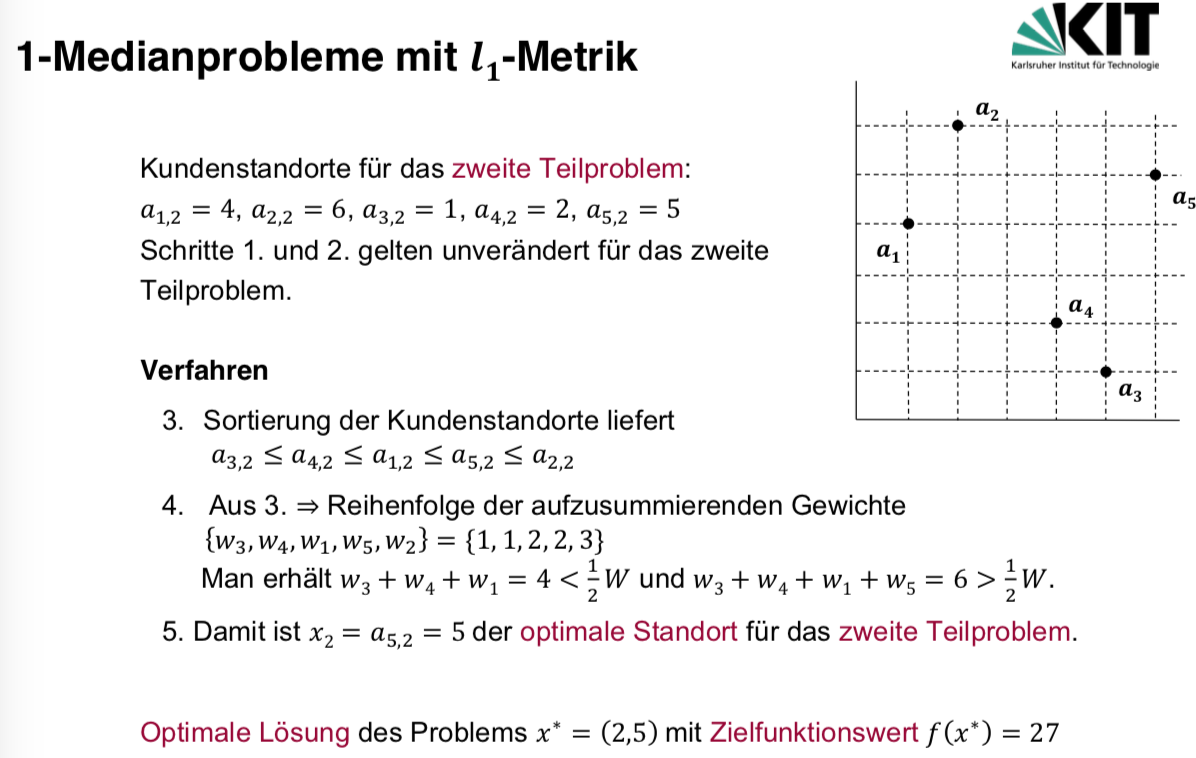
\includegraphics[width=0.95\textwidth]{Images/Loesungsverfahren_fuer_ungewichtete_1_Centreprobleme_Bsp.png}
            % \caption{Lösungsverfahren für ungewichtete 1-Centreprobleme mit $l_{\infty}$-Metrik}
            % \label{fig:Lösungsverfahren für ungewichtete 1-Centreprobleme mit l_{\infty}-Metrik}
          \end{figure}

        \subsubsubsection{Der allgemeine geweichtete Fall}

          \par \textbf{Zielfunktion}

          \begin{equation}
            \begin{aligned}
              g(x) &= \underset{i = 1, \dots, n}{\text{max}}w_i\text{max}\{|x_1 - a_{i,1}|, |x_2 - a_{i,2}|\} \\
                   &= \text{max}\{\underbrace{\underset{i = 1,\dots,n}{\text{max}}w_i|x_1 - a_{i,1}|}_{g_1(x_1}, \underbrace{\underset{i = 1,\dots,n}{\text{max}}w_i|x_2 - a_{i,2}|}_{g_2(x_2}\}
            \end{aligned}
          \end{equation}

          \par $\Rightarrow$ Das $l_{\infty}$-Centerproblem lässt sich in zwei voneinander unabhängige Teilprobleme zerlegen.


          \par \textbf{Das 1-Centerproblem mit $l_{\infty}$-Metrik auf der Linie}

          \[
            \underset{x \in \mathbb{R}}{\text{min}}g(x) \text{ mit } g(x) := \underset{i = 1, \dots, n}{\text{max}}w_i|x-a_i|
          \]
          \begin{algorithm}[H]
            \caption{Lösungsverfahren für gewichtete 1-Centreprobleme mit $l_{\infty}$-Metrik auf der Linie}
            % \textbf{Input}: Anzahl Suchrichtungen $K, \beta, V, p$
            \begin{algorithmic}[1]
              % \Procedure{MyProcedure}{}
              \State Berechne für jedes $i$ und $j$ mit $i, j \in {1, \dots, n}$
              \begin{equation*}
                \delta_{ij} = \frac{w_iw_j}{w_i+w_j}(a_j - a_i)
              \end{equation*}
              (Es gilt: $\delta_{ij} = -\delta{ji} \Rightarrow $ Es reicht aus, $\delta_{ij}$ oder $\delta_{ji}$ zu berechnen; je nachdem ob $a_i \leq a_j$ oder $a_i > a_j$)
              \State Ermittle 
              \begin{equation*}
                \delta_{pq} = max\{\delta_{ij}: i, j \in \{1, \dots, n\}\}
              \end{equation*}
              \State Optimal Lösung:
              \begin{equation*}
                z^* = \delta_{pq} \text{ und } x^{*} = \frac{w_pa_p + w_qa_q}{w_p + w_q}
              \end{equation*}
              
              % \EndProcedure
            \end{algorithmic}
            % \textbf{Output:} 
          \end{algorithm}

          \begin{exmp}
            
          \end{exmp}

          \begin{figure}[htbp]
            \centering
            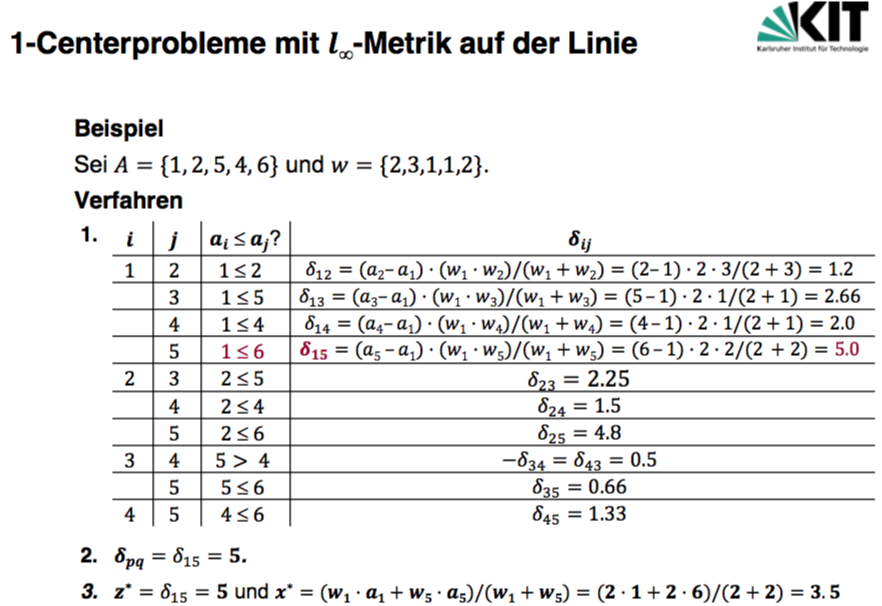
\includegraphics[width=0.95\textwidth]{Images/Das_1_Centerproblem_auf_der_Linie_Bsp.png}
            \caption{Das 1-Centerproblem mit $l_{\infty}$-Metrik auf der Linie}
            % \label{fig:Das 1-Centerproblem mit $l_{\infty}$-Metrik auf der Linie}
          \end{figure}

          \par \textbf{Kombination der Lösungen der Einzelprobleme}

          \par Seien $(x_1^*, z_1^*)$ und $(x_2^*, z_2^*)$ optimale Lösungen der zwei Teilprobleme.

          \par Dann ist $x^* := (x_1^*, x_2^*)$ eine optimale Lösungen mit $z^* = g(x^*) = \text{max}{\{g(x_1^*), g(x_2^*)\}} = \text{max}{\{z_1^*, z_2^*\}}$.

          \par Menge aller optimalen Lösungen ist

          \begin{equation*}
            \begin{aligned}
              \mathcal{X}^*(g) &= \mathcal{X}^*(g_1) \times \mathcal{X}^*(g_2) \\
                               &= [A_1^-(z^*), A_1^+(z^*)] \times [A_2^-(z^*), A_2^+(z^*)]
            \end{aligned}
          \end{equation*}
          \begin{itemize}
            \item $A^-(z) := \underset{i = 1,\dots, n}{\text{max}}a_i - \frac{z}{a_i}$
            \item $A^+(z) := \underset{i = 1,\dots, n}{\text{max}}a_i + \frac{z}{a_i}$
          \end{itemize}
      % subsubsection ungewichtete_1_centerprobleme_mit_ (end)
    
    % subsection 1_centerprobleme_mit_l_1_metrik (end)

    \subsection{1-Centerprobleme mit $l_2$-Metrik} % (fold)
    \label{sub:1_centerprobleme_mit_l_2_metrik}

      \subsubsection{Zielfunktion} % (fold)
      \label{ssub:zielfunktion}
        \begin{equation}
          \begin{aligned}
            g(x) &= \underset{i = 1,\dots, n}{\text{max}}w_il_2(x,a_i) \\
                 &= \underset{i = 1,\dots, n}{\text{max}}w_i\sqrt{(x_1 - a_{i, 1})^2 + (x_2 - a_{i,2})^2}
          \end{aligned}
        \end{equation}
      % subsubsection zielfunktion (end)

      \subsubsection{Der ungewichtete Fall: Das Kreis-Überdeckungsproblem} % (fold)
      \label{ssub:der_ungewichtete_fall_das_kreis_überdeckungsproblem}
        \par Umformulierung des Problems:

        \[
          \underset{x \in \mathbb{R}^2}{\text{min}} \underset{i = 1,\dots, n}{\text{max}}w_il_2(x,a_i) \Leftrightarrow \text{min } z, \text{u.d.N. } l_2(x, a_i) \leq z, \forall i = 1, \dots, n
        \]

        \par $\Rightarrow$ \textbf{Das minimale Kreis-Überdeckungsproblem}: Minimiere $z$ unter der Nebenbedingung, dass die Entfernung von einem Punkt $x$ zu allen Kundenstandorten kleiner oder gleich $z$ ist.

        \begin{algorithm}[H]
          \begin{algorithmic}[1]
            \caption{Enumertations-Verfahren}
              \State Berechne alle minimalüberdeckenden Kreise von zwei oder drei Kundenstandorten $a_i, a_j$ und $a_k \in A$
              \State Verwirf alle so gewonnen minimalüberdeckenden Kreise, die nicht alle Kundenstandorten überdecken.
              \State Der verbleibende MÜK (Minimal Überdeckender Kreis) ist der MÜK für alle Kundenstandorten
              % \EndProcedure
            \end{algorithmic}
          % \textbf{Output:} 
        \end{algorithm}

        \par Komplexität:$O(n^4) \rightarrow$ zu langsam!

        \begin{algorithm}[H]
          \begin{algorithmic}[1]
            \caption{Verfahren von Elzinga \& Hearn}
            \State Starte mit dem MÜK zweier beliebiger Kundenstandorten $a$ und $b$
            \State Werden alle Kunden von dem Kreis überdeckt $\Rightarrow$ Schritt 9
            \State Wähle einen Kunden $c$, der noch nicht überdeckt wird, und konstruiere den MÜK für diese drei Kunden.
            \State Werden alle Kunden von dem Kreis überdeckt $\Rightarrow$ Schritt 9.
            \State Wird der MÜK von zwei Kunden $a$ und $b$ bestimmt
              $\Rightarrow$ fahre mit $a$ und $b$ fort mit Schritt 3, 
              $\Rightarrow$ andernfalls fahre mit allen dreien fort mit Schritt 6.
            \State Wähle einen weiteren Kunden $d$, der noch nicht überdeckt wird, und konstruiere (mit Hilfe des Enumerations-Verfahrens) den MÜK für diese vier Kunden.  
            \State Werden alle Kunden von dem Kreis überdeckt $\Rightarrow$ Schritt 9
            \State Wird der MÜK von zwei Kunden $a$ und $b$ bestimmt
              $\Rightarrow$ fahre mit $a$ und $b$ fort mit Schritt 3, 
              $\Rightarrow$ andernfalls fahre mit den drei MÜK-definierenden Kunden fort mit Schritt 6.
            \State Der momentane MÜK überdeckt alle Kundenstandorte und ist somit der optimale.
              % \EndProcedure
            \end{algorithmic}
          % \textbf{Output:} 
        \end{algorithm}

        \begin{exmp}
          
        \end{exmp}

        \begin{figure}[H]
          \centering
          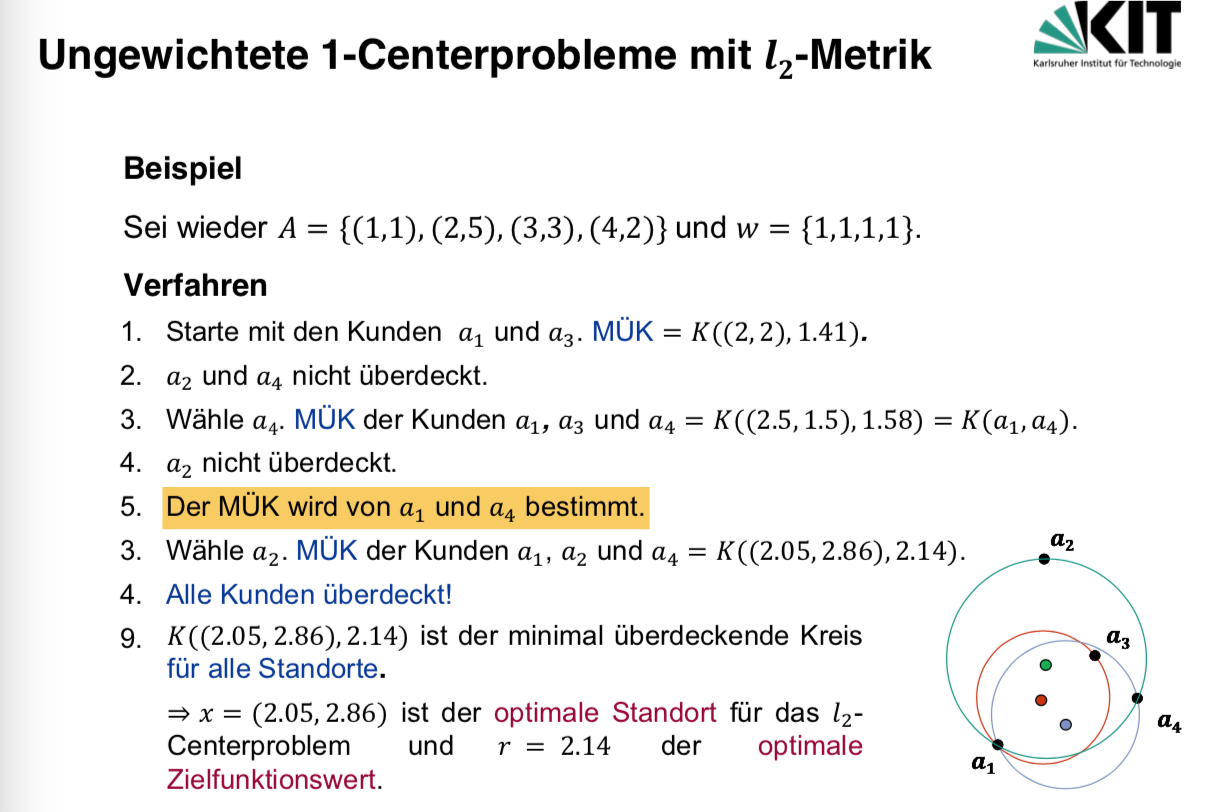
\includegraphics[width=0.95\textwidth]{Images/Verfahren_von_Elzinga_und_Hearn_Bsp.png}
          \caption{Verfahren von Elzinga \& Hearn}
          \label{fig:Verfahren von Elzinga & Hearn}
        \end{figure}

      % subsubsection der_ungewichtete_fall_das_kreis_überdeckungsproblem (end)
    
    % subsection 1_centerprobleme_mit_l_2_metrik (end)

  
  % section 1_centerprobleme (end)

  \section{Mehrstandortprobleme} % (fold)
  \label{sec:mehrstandortprobleme}

    \par Platziere $p$ neue Einrichtungen $X={x_1, \dots, x_p}, p \geq 2$ in der Ebene

    \begin{itemize}
      \item Modellen mit Interaktion
        \begin{itemize}
          \item Neue Einrichtungen bieten jeweils unterschiedlichen Service (verschiedene Güter) an.
          \item Kunden haben Nachfrage nach unterschiedlichen Serviceleistungen (Gütern) von mehreren der neuen Einrichtungen.
          \item Interaktion, z. B. Austausch von Gütern, zwischen neuen Einrichtungen erlaubt.
        \end{itemize}
      \item Zuordnungs-Modellen (Standort-Einzugsbereichs-Modellen
        \begin{itemize}
          \item Neue Einrichtungen bieten alle gleichen Service (identische Güter) an.
          \item Kunden befriedigen ihre Nachfrage von einem der neuen Standorte.
        \end{itemize}
    \end{itemize}
  
    \subsection{Modelle mit Interaktion} % (fold)
    \label{sub:modelle_mit_interaktion}

      \subsubsection{Annahmen} % (fold)
      \label{ssub:annahmen}

        \par \textbf{Nachfrage} des Kunden $i$ nach einem Service der neuen Einrichtung $k$: $w_ik$
        \par \textbf{Interaktion} zwischen zwei neuen Einrichtungen $k$ udn $l$: $s_{kl}$     
        % subsubsection annahmen (end)

      \subsubsection{Zielfunktion} % (fold)
      \label{ssub:zielfunktion}
      
        \begin{equation}
          \begin{aligned}
            \underset{X \subseteq \mathbb{R}^2, |X| = p}{\text{min}}f(X):= \sum_{i = 1}^{n}\sum_{k = 1}^{p}w{ik}d(x_k, a_i) + \sum_{k = 1}^{p - 1}\sum_{l = k + 1}^{p}s_{kl}d(x_k, x_l)    
          \end{aligned}
        \end{equation}
      % subsubsection zielfunktion (end)

      \subsubsection{Notationen} % (fold)
      \label{ssub:notationen}

        \par $x_1, \dots, x_p$ sind nun Punkte mit Koordinaten $x_{k,1}$ und $x_{k,2}, k = 1, \dots, p$

        \par $X_1:= {x_{1,1}, \dots, x_{p,1}}$ und $X_2 := {x_{1,2}, \dots, x_{p,2}}$
      
      % subsubsection notationen (end)

      \subsubsection{Das Interaktions-Modell mit $l_1$-Metrik} % (fold)
      \label{ssub:das_interaktions_modell_mit_l1_metrik}

      \par \textbf{Zielfunktion}

      \begin{equation}
        \begin{aligned}
          f(X) &= \sum_{i=1}^{n}\sum_{k=1}^{p}w_{ik}(|x_{k,1}-a_{i,1}| + |x_{k,2}- a_{i,2}|) + \sum_{k=1}^{p-1}\sum_{l=k+1}^{p}s_{kl}(|x_{k,1}-x_{l,1}|+|x_{k,2}- x_{l,2}|) \\
               &=  \underbrace{\sum_{i=1}^{n}\sum_{k=1}^{p}w_{ik}|x_{k,1}-a_{i,1}| + \sum_{k=1}^{p-1}\sum_{l=k+1}^{p}s_{kl}|x_{k,1}-x_{l,1}|}_{=: f_1(X_1)} + \underbrace{\sum_{i=1}^{n}\sum_{k=1}^{p}w_{ik}|x_{k,2}-a_{i,2}| + \sum_{k=1}^{p-1}\sum_{l=k+1}^{p}s_{kl}|x_{k,2}-x_{l,2}|}_{f_2(X_2)}
        \end{aligned} 
      \end{equation}

      $\rightarrow$Zielfunktion zerfällt in zwei voneinander unabhängige Funktionen.

      \par \textbf{Das Interaktions-Modell mit $l_1$-Metrik auf der Linie}

      \par \textbf{Zielfunktion}

      \begin{equation}
        \sum_{i=1}^{n}\sum_{k=1}^{p}w_{ik}|x_{k}-a_{i}| + \sum_{k=1}^{p-1}\sum_{l=k+1}^{p}s_{kl}|x_{k}-x_{l}|
      \end{equation}

      \par \textbf{Umformulierung}

      \begin{framed}
        \par Seien $a, b \in \mathbb{R}$ und $c, d \in \mathbb{R}_+$\\
        \par Gilt: 
        \[c \cdot d = 0 \text{ und } a - b = c - d\]
        \par Dann:
        \[|a - b| = c + d\]
        \par Ersetze:
        \[|x_k - a_i| = \alpha_{ik} + \beta_{ik} \in \mathbb{R}_+, \text{für } \alpha_{ik}, \beta_{ik} \in \mathbb{R}_+\]
        \par und 
        \[|x_k - x_l| = \gamma_{kl} + \delta_{kl} \in \mathbb{R}_+, \text{für } \in \gamma_{kl}, \delta_{kl} \in \mathbb{R}_+\]
      \end{framed}
      
      % subsubsection das_interaktions_modell_mit_l1_metrik (end)
    
    % subsection modelle_mit_interaktion (end)

    \section{Zuordnungs-Modelle} % (fold)
    \label{sub:zuordnungs_modelle}
    
    % section zuordnungs_modelle (end)

  % section mehrstandortprobleme (end)


% chapter standortplanung_in_der_ebene (end)


